\documentclass[conference,a4paper]{IEEEtran}

\usepackage[utf8]{inputenc}
\usepackage[T1]{fontenc}
\usepackage[brazil]{babel}
\usepackage{cite}
\usepackage{amsmath}
\usepackage{booktabs}
\usepackage{array}
\usepackage{tabularx}
\usepackage{graphicx}
\usepackage{xcolor}
\usepackage{tikz}
\usetikzlibrary{arrows.meta,positioning}
\usepackage{acro}
\usepackage{microtype}
\usepackage{xurl}
\usepackage[hidelinks]{hyperref}

\acsetup{first-style=short}
\DeclareAcronym{v2x}{short=V2X,long=comunicação entre veículos e outros elementos do trânsito}
\DeclareAcronym{v2v}{short=V2V,long=comunicação entre veículos}
\DeclareAcronym{v2i}{short=V2I,long=comunicação entre veículo e infraestrutura}
\DeclareAcronym{icrw}{short=ICRW,long=Intersection Collision Risk Warning}
\DeclareAcronym{los}{short=LOS,long=line of sight}
\DeclareAcronym{nlos}{short=NLOS,long=non-line of sight}
\DeclareAcronym{cam}{short=CAM,long=Cooperative Awareness Message}
\DeclareAcronym{denm}{short=DENM,long=Decentralized Environmental Notification Message}
\DeclareAcronym{rsu}{short=RSU,long=roadside unit}
\DeclareAcronym{gnss}{short=GNSS,long=Global Navigation Satellite System}
\DeclareAcronym{pdr}{short=PDR,long=packet delivery ratio}
\DeclareAcronym{hil}{short=HIL,long=hardware-in-the-loop}
\newcolumntype{Y}{>{\raggedright\arraybackslash}X}
\newcommand{\un}[1]{\,\mathrm{#1}}
\newcommand{\changed}[1]{{#1}}
\setlength{\emergencystretch}{1em}

\title{Comunicação V2X para alertas de colisão em cruzamentos sem visada direta: estudo de caso e análise dos requisitos de rede}
\author{\IEEEauthorblockN{Álvaro Lucio Almeida Ribeiro e Matheus Henrique Fonseca Afonso}
\IEEEauthorblockA{Curso de Mestrado, Instituto Nacional de Telecomunicações -- Inatel\\
Santa Rita do Sapucaí, MG, Brasil\\
TP546 -- Internet das Coisas e Redes Veiculares\\
Professor: Samuel Baraldi Mafra}}
\hypersetup{pdftitle={Comunicação V2X para alertas de colisão em cruzamentos sem visada direta},
pdfauthor={Álvaro Lucio Almeida Ribeiro e Matheus Henrique Fonseca Afonso},
pdfsubject={Estudo de caso -- TP546},pdfkeywords={redes veiculares, V2X, cruzamentos, latência, confiabilidade}}

\begin{document}
\pagestyle{plain}
\maketitle
\thispagestyle{plain}

\begin{abstract}
Em cruzamentos com obstáculos, dois veículos podem aproximar-se de uma mesma região de conflito antes que seus condutores tenham contato visual. A comunicação entre veículos e outros elementos do trânsito (V2X) permite compartilhar estados de movimento e antecipar alertas, mas sua utilidade depende da chegada de informações confiáveis dentro do tempo disponível para reação. Este trabalho apresenta um estudo bibliográfico sobre alertas de colisão em cruzamentos sem visada direta. Um estudo experimental publicado é examinado em conjunto com uma avaliação que integra equipamentos reais e simulação, especificações de mensagens e requisitos de aplicação. A análise distingue desempenho do enlace, atualidade da informação e oportunidade do alerta. Um exemplo analítico próprio relaciona velocidade, atraso e distância de parada, sem representar uma medição de campo. Também se organiza um roteiro de avaliação que inclui perdas consecutivas, erros de localização e falsos alertas. A síntese indica que a taxa média de entrega de pacotes é insuficiente para caracterizar o serviço: é necessário verificar quando o estado remoto deixa de ser válido e quanto tempo resta para uma resposta. As conclusões limitam-se aos cenários e às versões tecnológicas examinados, sem estabelecer uma superioridade universal entre tecnologias de acesso nem comprovar redução de acidentes em vias públicas.
\end{abstract}

\begin{IEEEkeywords}
redes veiculares, V2X, alerta de colisão, cruzamentos, latência, confiabilidade.
\end{IEEEkeywords}

\section{Introdução}
Uma edificação na esquina pode ocultar um veículo que se aproxima por uma via transversal. Nesse caso, observar somente o espaço visível à frente não informa ao condutor se outro participante chegará ao cruzamento no mesmo instante. O problema combina oclusão, mobilidade e um intervalo limitado para decidir. A comunicação \ac{v2x}, do inglês \textit{vehicle-to-everything}, permite que estados de movimento sejam recebidos antes do contato visual, oferecendo uma entrada adicional à avaliação de risco.

\changed{A Figura~\ref{fig:cruzamento} representa a oclusão entre dois veículos em aproximação e situa a região em que suas trajetórias podem entrar em conflito.}

\begin{figure}[t]
\centering
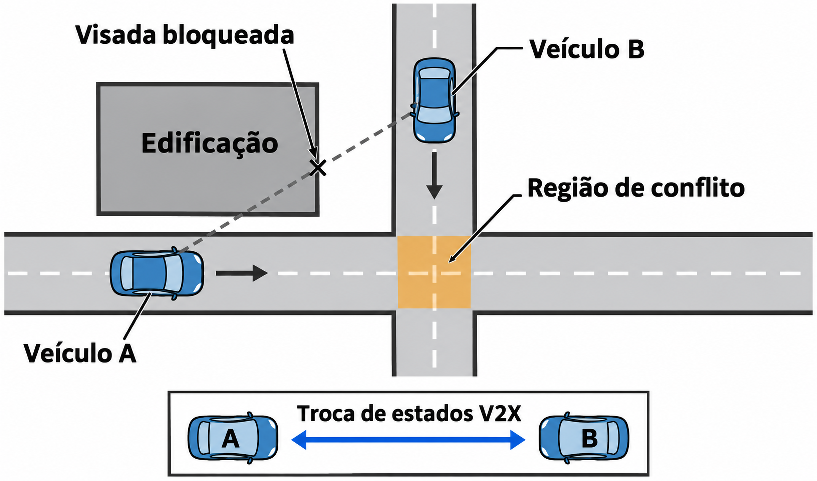
\includegraphics[width=\columnwidth]{images/cruzamento_obstruido.pdf}
\caption{\changed{Cruzamento com visada obstruída por uma edificação. A e B aproximam-se da região de conflito. O quadro inferior representa a troca conceitual de estados, sem descrever um percurso de propagação nem garantir recepção. Elaboração própria.}}
\label{fig:cruzamento}
\end{figure}

A Figura~\ref{fig:rodovia} ilustra a comunicação entre veículos em uma rodovia. Os círculos representam conectividade de maneira conceitual, sem indicar alcance ou confiabilidade medidos. Neste trabalho, o foco se restringe a cruzamentos urbanos, onde edificações e outros veículos podem limitar a observação das trajetórias transversais.

\begin{figure}[t]
\centering
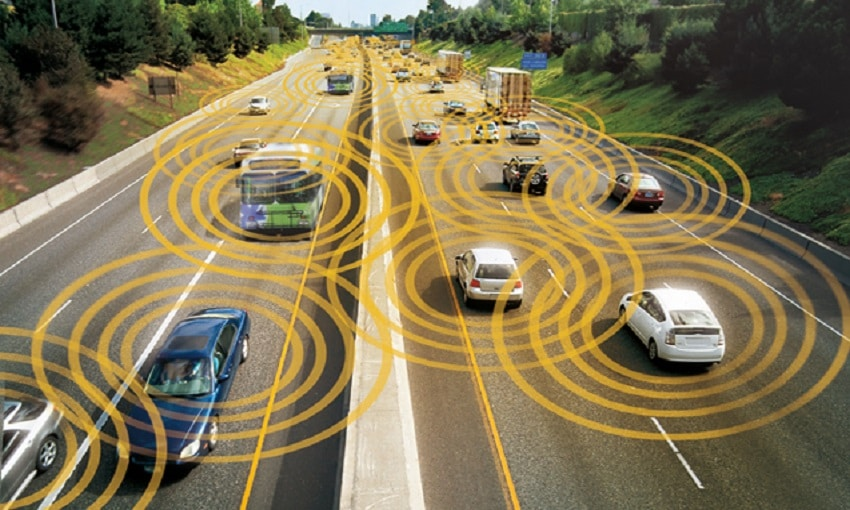
\includegraphics[width=\columnwidth]{images/imagem.jpg}
\caption{Representação conceitual de veículos conectados em uma rodovia. Crédito: U.S. Department of Transportation, conforme a publicação da GovTech~\cite{veen2014}.}
\label{fig:rodovia}
\end{figure}

O alerta de risco de colisão em cruzamentos, denominado \ac{icrw}, é uma aplicação especificada pela ETSI~\cite{etsiICRW2018}. O interesse deste trabalho é o conflito entre veículos em trajetórias transversais, com obstrução da visada direta. A sigla \ac{los} indica uma situação com visada, enquanto \ac{nlos} indica sua ausência. Essa delimitação permite estudar uma aplicação concreta, em vez de tratar indistintamente todas as funções de transporte inteligente.

Comunicar além do campo visual não equivale a garantir observação contínua. O receptor pode receber uma posição antiga, interpretar uma faixa incorretamente ou perder atualizações durante a aproximação. Uma comunicação rápida também pode chegar tarde se a primeira informação útil surgir quando a distância restante já for insuficiente. Por isso, a pergunta orientadora é: quais propriedades da rede precisam ser avaliadas para que um alerta cooperativo seja útil em um cruzamento sem visada direta?

O objetivo é relacionar as evidências de um caso experimental aos requisitos de uma cadeia completa de alerta. A contribuição é didática e analítica: separar o que foi publicado, o que pode ser deduzido sob hipóteses explícitas e o que ainda precisaria de validação. A análise utiliza estudos com comunicação LTE veicular e ITS-G5.

O argumento central é que a avaliação deve acompanhar a informação desde sua obtenção até a apresentação do aviso. O sucesso de uma transmissão descreve uma etapa dessa cadeia. A utilidade para o condutor exige, adicionalmente, estado relevante, trajetória plausível e tempo de resposta. As seções seguintes apresentam o método, os fundamentos, os casos selecionados, um modelo ilustrativo e os critérios de avaliação derivados dessa perspectiva.

\section{Método e delimitação do estudo}
\subsection{Seleção e função das fontes}
Adota-se uma revisão narrativa com estudo de caso. A seleção foi orientada por três necessidades: encontrar uma aplicação explicitamente ligada a cruzamentos, dispor de resultados verificáveis e identificar requisitos técnicos que permitissem interpretar esses resultados. Não se trata de revisão sistemática, levantamento exaustivo ou metanálise. As fontes foram consultadas em novembro de 2026.

O estudo de Wang et al.~\cite{wang2021} fornece o caso experimental com a plataforma CAVTest. A avaliação de Bazzi et al.~\cite{bazzi2020} acrescenta evidência de integração entre tráfego, equipamentos e canal emulado. Gonzalez-Martin et al.~\cite{gonzalez2019} fundamentam a discussão sobre acesso autônomo ao meio. As especificações ETSI e 3GPP~\cite{etsiICRW2018,etsiCAM2019,etsiSecurity2017,3gpp2024} são empregadas para interpretar funções e interfaces, e não como prova de desempenho de um produto.

As versões das especificações são registradas nas referências, sem pressupor que sejam as mais recentes ou que tenham sido integralmente implementadas nos experimentos. A arquitetura conceitual organiza funções comuns, sem atribuir mensagens europeias à pilha de outro país nem afirmar compatibilidade entre os sistemas citados.

\subsection{Critérios de interpretação}
As evidências são separadas em três níveis: observações reportadas pelos autores dos experimentos, requisitos e formatos documentados por organismos de padronização, e cálculos ilustrativos e recomendações analíticas deste trabalho. Essa distinção separa resultados medidos, metas de projeto e relações físicas simplificadas.

A comparação entre fontes é qualitativa, pois os estudos diferem em ambiente, tecnologia, geometria, algoritmo e comportamento dos condutores. Não se agregam percentuais de sucesso nem se classificam tecnologias. A unidade de análise é a relação entre condição de comunicação e oportunidade do alerta.

O escopo contempla condutores humanos e avisos de assistência. Frenagem automática, coordenação de trajetórias e condução autônoma exigiriam requisitos adicionais de controle e validação. Também não se estima o número de acidentes evitados por uma implantação comercial. Essa estimativa dependeria de exposição ao risco, adesão da frota, comportamento humano e observações prolongadas, indisponíveis no presente estudo.

\section{Fundamentos da aplicação cooperativa}
\subsection{Comunicação direta e apoio da infraestrutura}
A comunicação \ac{v2v}, do inglês \textit{vehicle-to-vehicle}, liga participantes móveis, enquanto a comunicação \ac{v2i}, ou \textit{vehicle-to-infrastructure}, envolve equipamentos viários. Uma unidade de acostamento, \ac{rsu}, pode apoiar o serviço. Na arquitetura LTE veicular, a interface PC5 permite comunicação direta e a interface LTE-Uu conecta o terminal à rede celular. A especificação 3GPP TS 23.285 também contempla operações que combinam esses caminhos~\cite{3gpp2024}.

A Figura~\ref{fig:interfaces} situa essas modalidades ao lado da comunicação com pedestres (V2P) e com a rede (V2N). O diagrama organiza os participantes, mas não determina o caminho efetivo de cada mensagem nem a tecnologia de acesso empregada.

\begin{figure}[t]
\centering
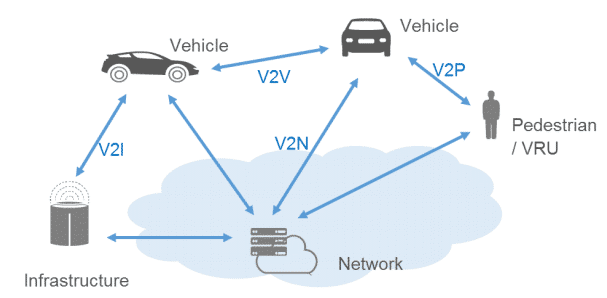
\includegraphics[width=\columnwidth]{images/imagem2.png}
\caption{Modalidades de comunicação V2X. Diagrama atribuído ao 3GPP na apresentação da Harris~\cite{harris2019}, slide 6, hospedada pelo NIST.}
\label{fig:interfaces}
\end{figure}

Essa separação importa para formular o cenário. Se duas unidades trocam estados diretamente, não se deve atribuir ao percurso da mensagem uma passagem obrigatória pela nuvem. Se a decisão depender de um servidor, seu caminho de comunicação precisa entrar no orçamento de atraso e na análise de disponibilidade. A palavra ``celular'', isoladamente, não identifica a sequência de componentes atravessada por cada atualização.

Gonzalez-Martin et al.~\cite{gonzalez2019} estudam o modo 4 de LTE-V2X, no qual os veículos selecionam recursos de rádio autonomamente, sem assistência da infraestrutura celular. Seus modelos tratam a entrega de pacotes em função de parâmetros de transmissão e densidade. A existência dessa seleção distribuída ajuda a compreender por que operar sem cobertura não elimina problemas de disputa por recursos. A análise é específica desse modo, sem extensão automática a outras configurações LTE ou ao NR-V2X.

No cenário conceitual deste artigo, a decisão ocorre no veículo receptor a partir de estados recebidos diretamente. Uma \ac{rsu} é considerada como possível complemento de observação e distribuição de informações. Sua inclusão deve responder a uma necessidade identificada, como um ponto cego persistente. Adicioná-la sem medir a cobertura e o percurso de processamento pode apenas deslocar o local onde a informação atrasa.

\subsection{Estado, evento e contexto viário}
O serviço europeu de consciência cooperativa utiliza mensagens \ac{cam}, que transportam informações como posição, velocidade e orientação. Na ETSI EN 302 637-2 V1.4.1, a geração veicular opera entre 100 e 1\,000~ms e considera a dinâmica do veículo e as condições de congestionamento. A mensagem é difundida em um salto e não deve ser retransmitida por uma estação receptora~\cite{etsiCAM2019}.

Um estado descreve o movimento observado em um instante. Um evento informa uma situação identificada pela aplicação. As mensagens \ac{denm} são notificações de eventos. A especificação de \ac{icrw} considera processamento de \ac{cam} e \ac{denm} e, quando aplicável, informações sobre semáforos e topologia~\cite{etsiICRW2018}. Esses papéis não autorizam tratar todo pacote de presença como um alerta nem supor que toda decisão exija transmissão adicional de evento.

Para interpretar o estado remoto, o receptor precisa associá-lo ao cruzamento correto e a um movimento compatível com o conflito. Dois veículos geograficamente próximos podem ocupar vias em níveis diferentes. Um veículo que se aproxima pode frear, virar ou permanecer parado. O mapa e o histórico ajudam a formular hipóteses de trajetória, mas não removem a necessidade de representar incerteza.

O sistema global de navegação por satélite, \ac{gnss}, oferece uma referência de posição e tempo. Para a aplicação, porém, importa a relação entre a posição estimada e a geometria da via. Um erro lateral pode mudar a faixa atribuída ao veículo, enquanto um erro longitudinal altera a previsão de chegada. Essa diferença sugere avaliar o erro na direção relevante ao conflito, em vez de registrar apenas uma média espacial única.

\begin{figure*}[t]
\centering
\begin{tikzpicture}[
box/.style={draw,rounded corners,align=center,text width=2.6cm,minimum height=1.05cm,font=\small},
arr/.style={-{Latex[length=2mm]},thick},node distance=0.7cm]
\node[box] (origem) {Veículo A\\posição, velocidade\\e instante de medição};
\node[box,right=of origem] (tx) {Formação e\\proteção da\\mensagem};
\node[box,right=of tx] (radio) {Acesso ao meio\\e canal de rádio\\com obstáculos};
\node[box,right=of radio] (rx) {Veículo B\\validação, atualização\\e previsão};
\node[box,right=of rx] (hmi) {Alerta ao condutor\\e tempo restante\\para reagir};
\draw[arr] (origem) -- (tx);
\draw[arr] (tx) -- (radio);
\draw[arr] (radio) -- (rx);
\draw[arr] (rx) -- (hmi);
\node[draw,dashed,align=center,font=\small,text width=5.0cm,below=0.7cm of rx] (rsu) {Apoio opcional da infraestrutura:\\observação local e contexto do cruzamento};
\draw[arr,dashed] (rsu) -- (rx);
\end{tikzpicture}
\caption{Cadeia funcional de um alerta cooperativo. Elaboração própria. O apoio da infraestrutura é uma alternativa de projeto, e não uma etapa obrigatória da comunicação direta.}
\label{fig:cadeia}
\end{figure*}

\subsection{Latência e idade da informação}
A Figura~\ref{fig:cadeia} organiza a cadeia funcional. Define-se a latência de aplicação como o intervalo entre a disponibilidade de um dado na origem e a apresentação de um aviso correspondente no destino. Essa definição inclui aquisição disponível ao sistema, formação da mensagem, acesso ao meio, recepção, validação, decisão e interface. Medir somente o percurso entre rádios responde a uma pergunta mais restrita.

Na ETSI TS 101 539-2 V1.1.1, o intervalo da disponibilidade do dado ao aviso é associado tipicamente a 300~ms~\cite{etsiICRW2018}. O valor não é apresentado aqui como prazo universal de qualquer cruzamento. Velocidade, geometria e política de alerta alteram a margem disponível. Tampouco esse intervalo deve ser confundido com um atraso exclusivo da interface sem fio.

Se a última amostra válida foi produzida em $t_g$ e a decisão ocorre em $t$, sua idade é
\begin{equation}
 A(t)=t-t_g.
 \label{eq:idade}
\end{equation}
Essa idade pode crescer mesmo quando os pacotes recebidos apresentam baixa latência, pois atualizações intermediárias podem ter sido perdidas. Também depende da qualidade da referência temporal. Se os relógios não estiverem alinhados, parte do valor observado pode ser erro de sincronização. Uma avaliação precisa declarar como esse erro foi controlado.

Uma consequência prática é distinguir ``último pacote recebido'' de ``último estado aceito''. Uma mensagem pode chegar, mas ser rejeitada por idade, autenticidade ou inconsistência. Manter o estado antigo após essa rejeição não equivale a obter informação nova. O registro experimental precisa mostrar ambos os eventos para que uma aparente continuidade de recepção não oculte uma interrupção de conhecimento útil.

\section{Estudo de caso e evidências complementares}
\subsection{Ensaio com a plataforma CAVTest}
Wang et al.~\cite{wang2021} avaliaram alertas com LTE-V em cruzamentos com visada, rurais e urbanos. No cenário com visada, foram consideradas comunicação sem degradação artificial e taxas de entrega impostas de 75\% e 25\%, com 100 repetições por combinação de velocidade e condição. O risco foi estimado pela proximidade dos tempos de chegada ao conflito.

Os autores distinguem alerta preciso (PW), que permite frenagem parcial, alerta efetivo (EW), que exige frenagem plena, e sucesso total (SW), soma de PW e EW. A Tabela~\ref{tab:caso} reúne resultados selecionados a 40~km/h sob o protocolo publicado. Sucesso total elevado pode coexistir com menor proporção de avisos antecipados.

\begin{table}[t]
\centering
\caption{Resultados publicados a 40~km/h. Seleção das Tabelas 3 e 4 de Wang et al.~\cite{wang2021}.}
\label{tab:caso}
\small
\begin{tabularx}{\columnwidth}{Yrrr}
\toprule
Condição & PW (\%) & EW (\%) & SW (\%)\\
\midrule
Com visada, sem degradação artificial & 98 & 2 & 100\\
Com visada, entrega imposta de 75\% & 52 & 46 & 98\\
Com visada, entrega imposta de 25\% & 20 & 66 & 86\\
Rural & 95 & 5 & 100\\
Urbana & 55 & 42 & 97\\
\bottomrule
\end{tabularx}
\end{table}

\subsection{Avaliação com equipamentos e canal emulado}
Bazzi et al.~\cite{bazzi2020} empregam uma plataforma \ac{hil}, que integra simulação de mobilidade, trocas reais ITS-G5 e emulação de canal. O cenário utiliza uma região urbana de Bolonha e veículos conduzidos por humanos. A aplicação examina tempos de chegada ao cruzamento, produz níveis de aviso e é avaliada por colisões simuladas e tempo de viagem. O estudo contrasta canais idealizados e canais com condições de propagação modeladas.

A conclusão pertinente é que considerar canal ideal pode produzir uma avaliação excessivamente favorável da segurança. O trabalho também explicita uma relação entre a resposta aos avisos e a eficiência do tráfego. Essa evidência complementa a pista fechada porque permite observar consequências da política de alerta ao longo de múltiplas interações. Não representa, contudo, observação de acidentes reais na cidade modelada.

Os dois tipos de avaliação respondem a perguntas diferentes. Em pista, a geometria física e os equipamentos participam diretamente da comunicação observada. Em \ac{hil}, parte do ambiente é controlada por modelos e parte da cadeia utiliza hardware. Nenhuma dessas propriedades, isoladamente, determina qual resultado deve prevalecer em outro local. A interpretação exige identificar exatamente o que foi medido, emulado ou pressuposto.

\subsection{Leitura crítica das evidências}
Para interpretar um resultado agregado, convém perguntar qual evento conta como sucesso. Evitar conflito sob frenagem intensa e avisar com antecedência confortável são objetivos relacionados, mas distintos. Uma decisão de implantação deveria registrar ambos, pois a classificação binária pode esconder diferenças no esforço solicitado ao condutor. Essa é uma escolha de avaliação que pode ser aplicada independentemente da tecnologia de rádio.

Também é necessário separar indisponibilidade do enlace de indisponibilidade do serviço. O enlace pode falhar em um instante sem prejudicar a decisão, caso exista uma estimativa recente e confiável. Inversamente, a recepção pode continuar enquanto a aplicação associa o estado à trajetória errada. A avaliação deve localizar a falha na cadeia antes de atribuí-la a uma suposta limitação da tecnologia.

Uma comparação direta entre LTE-V e ITS-G5 exigiria controlar distâncias, potência, instalação das antenas, densidade, mensagens e limiares de decisão. Como os estudos não compartilham esse protocolo experimental, sua leitura conjunta mostra formas complementares de avaliar a aplicação.

\section{Análise ilustrativa da margem de reação}
\subsection{Hipóteses e definição do conflito}
Para tornar explícita a relação entre rede e movimento, considera-se um exemplo próprio: dois veículos aproximam-se de um cruzamento perpendicular em trajetórias previamente conhecidas. Durante o horizonte curto de previsão, cada veículo mantém velocidade positiva constante até o início da reação. Não há aceleração longitudinal prévia, mudança de faixa ou incerteza de mapa. Essas simplificações servem à análise, sem reproduzir integralmente os algoritmos dos estudos citados.

Se $d_i$ é a distância ao início da região de conflito e $v_i$ é a velocidade, o tempo previsto de chegada é
\begin{equation}
 \tau_i=\frac{d_i}{v_i},\qquad v_i>0.
 \label{eq:chegada}
\end{equation}
A diferença $|\tau_A-\tau_B|$ pode indicar proximidade temporal, mas não descreve sozinha o conflito. Os veículos ocupam espaço e levam tempo para atravessar a região compartilhada. Uma avaliação mais coerente considera intervalos de ocupação, em vez de tratar ambos como pontos sem dimensão.

Se $\ell_i$ representa o percurso necessário para que o veículo libere a região, incluindo seu comprimento, define-se
\begin{equation}
 I_i=\left[\tau_i,\;\tau_i+\frac{\ell_i}{v_i}\right].
\end{equation}
A interseção $I_A\cap I_B\ne\emptyset$ indica um conflito potencial sob as hipóteses adotadas. Isso não é uma probabilidade de colisão. Alterações de velocidade, prioridade e intenção podem modificar os intervalos. Para veículos parados ou muito lentos, a divisão por velocidade torna-se inadequada e outro modelo de estado é necessário.

\changed{A Figura~\ref{fig:decisao} organiza a validação, a previsão de ocupação e os resultados possíveis de um ciclo de avaliação. Uma mensagem nova rejeitada pode coexistir com um estado anterior ainda válido. O teste de disponibilidade considera esse estado e sua idade, inclusive nos ciclos sem novas mensagens.}

\begin{figure*}[t]
\centering
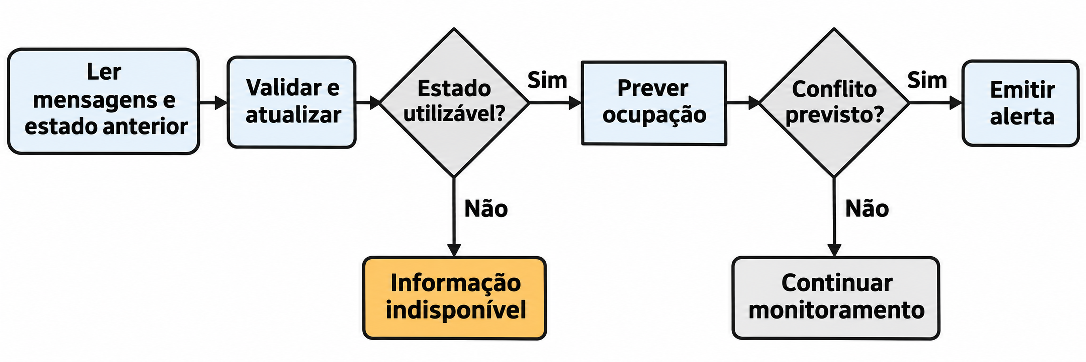
\includegraphics[width=\textwidth]{images/fluxograma_alerta.pdf}
\caption{\changed{Fluxo conceitual de avaliação do alerta, elaborado a partir das funções discutidas no estudo. A disponibilidade é verificada sobre o estado mantido após a validação. A ausência de estado utilizável conduz à informação indisponível, enquanto a ausência de conflito previsto conduz à continuidade do monitoramento. Elaboração própria, sem implementação experimental associada.}}
\label{fig:decisao}
\end{figure*}

\subsection{Atraso convertido em distância}
Se o veículo mantém velocidade $v$ durante uma espera $T$, percorre $vT$. Sob frenagem constante de magnitude $a>0$, a distância posterior de frenagem é $v^2/(2a)$. Logo, uma aproximação da distância necessária desde o instante em que a informação fica disponível na origem é
\begin{equation}
 D=v(L+R)+\frac{v^2}{2a},
 \label{eq:parada}
\end{equation}
em que $L$ agrega a espera até o aviso e $R$ agrega reação humana e início da frenagem. Esse modelo não inclui inclinação, variação de aderência ou crescimento gradual da desaceleração. Ele também não é usado para prescrever uma distância segura de operação.

Adotam-se, somente para ilustração, $R=1{,}5\un{s}$ e $a=4\un{m/s^2}$. Esses valores são hipóteses deste trabalho, não parâmetros medidos nem recomendações normativas. A Tabela~\ref{tab:distancia} apresenta os cálculos. O termo $L$ assume 0,1 e 0,3~s como exemplos numéricos de espera total, sem atribuí-los ao desempenho de uma tecnologia.

\begin{table}[t]
\centering
\caption{Distância calculada pela Eq.~\eqref{eq:parada}, com $R=1{,}5\un{s}$ e $a=4\un{m/s^2}$. Elaboração própria.}
\label{tab:distancia}
\small
\setlength{\tabcolsep}{4pt}
\begin{tabular}{rrrr}
\toprule
$v$ (km/h) & $D$, $L=0{,}1$ s (m) & $D$, $L=0{,}3$ s (m) & Diferença (m)\\
\midrule
30 & 22,01 & 23,68 & 1,67\\
40 & 33,21 & 35,43 & 2,22\\
50 & 46,33 & 49,11 & 2,78\\
\bottomrule
\end{tabular}
\end{table}

A 40~km/h, acrescentar 0,2~s à espera consome cerca de 2,22~m. Esse acréscimo não muda a distância de frenagem do modelo, mas reduz o espaço disponível antes dela. O efeito ilustra por que uma diferença temporal aparentemente pequena pode importar perto do limite de reação. Em contrapartida, reduzir o atraso não compensa necessariamente uma observação inicial feita tarde demais.

Para uma distância disponível $d$, a margem do modelo é $M=d-D$. Um valor negativo informa que as hipóteses adotadas não permitem a parada completa antes do conflito. Um valor positivo não garante segurança real, pois o modelo omite incertezas e outros movimentos. A utilidade da margem está em revelar quais hipóteses produzem a conclusão, permitindo questioná-las antes de interpretar o resultado como proteção efetiva.

\subsection{Perdas consecutivas e estado desatualizado}
Considere-se uma sequência hipotética de atualizações a cada $T=0{,}1\un{s}$, sem atraso de geração variável. Com $k$ mensagens consecutivas perdidas, a idade imediatamente antes da próxima recepção pode aproximar-se de $(k+1)T+L_r$, em que $L_r$ é a latência de transporte da atualização seguinte. A expressão é uma contabilidade temporal simplificada, não um modelo estatístico do canal.

Duas sequências com a mesma quantidade de pacotes recebidos podem produzir idades muito diferentes. Se as perdas estiverem espalhadas, uma atualização recente pode aparecer entre elas. Se estiverem concentradas junto ao cruzamento, o receptor pode permanecer sem observação útil justamente durante o conflito. Por isso, a média da entrega não informa a duração da pior interrupção nem sua posição na trajetória.

Em um cenário idealizado de recepções independentes, com probabilidade $p$ por mensagem, a probabilidade de pelo menos uma recepção em $n$ tentativas é
\begin{equation}
 P_{\geq 1}=1-(1-p)^n.
\end{equation}
A expressão deixa visível o benefício potencial de múltiplas oportunidades, mas a independência é uma hipótese forte. Uma obstrução persistente ou um conflito recorrente de recursos pode afetar várias transmissões seguidas. Não se usa essa equação para estimar a confiabilidade do caso experimental nem para converter entrega de pacotes diretamente em prevenção de colisões.

\changed{Para quantificar o efeito da ordem das perdas, considera-se um exemplo determinístico próprio com 20 mensagens geradas nos instantes $t_j=jT$, para $j=1,\ldots,20$, durante $H=2\un{s}$. Admite-se um estado válido em $t=0$, relógios sincronizados e recepção instantânea das mensagens entregues. No padrão disperso, perdem-se as mensagens de índices 4, 8, 12 e 16. Na rajada, perdem-se as de índices 8, 9, 10 e 11. Ambos entregam 16 das 20 mensagens, com \ac{pdr} de 80\%.}

\changed{Além do pico da idade, calculam-se sua média temporal $\overline{A}$ e a fração $Q_\theta$ do período observado em que a idade excede um limiar $\theta$:}
\begin{equation}
\begin{aligned}
\overline{A}&=\frac{1}{H}\int_0^H A(t)\,\mathrm{d}t,\\
Q_\theta&=\frac{1}{H}\int_0^H\mathbf{1}_{\{A(t)>\theta\}}\,\mathrm{d}t.
\end{aligned}
\label{eq:violacao-idade}
\end{equation}
\changed{A função indicadora vale um quando a condição é satisfeita e zero nos demais instantes. Adota-se $\theta=0{,}25\un{s}$ apenas como parâmetro ilustrativo. Esse limiar se refere à idade do estado e não ao intervalo entre disponibilidade do dado e aviso discutido anteriormente.}

\begin{table}[t]
\centering
\caption{Efeito da distribuição de quatro perdas em 20 mensagens. Cálculo determinístico próprio com $T=0{,}1\un{s}$ e latência de transporte nula.}
\label{tab:padroes-perda}
\small
\begin{tabularx}{\columnwidth}{Yrr}
\toprule
Indicador & Dispersas & Rajada\\
\midrule
\ac{pdr} (\%) & 80 & 80\\
Maior intervalo entre recepções (ms) & 200 & 500\\
Pico da idade (ms) & 200 & 500\\
Idade média $\overline{A}$ (ms) & 70 & 100\\
Fração $Q_{0{,}25\,\mathrm{s}}$ (\%) & 0 & 12,5\\
\bottomrule
\end{tabularx}
\end{table}

\changed{Como a idade cresce linearmente entre recepções e retorna a zero em cada entrega, um intervalo de duração $g$ contribui com área $g^2/2$ para sua integral. O padrão disperso possui quatro intervalos de 0,2~s e doze de 0,1~s. A rajada produz um intervalo de 0,5~s e quinze de 0,1~s. Nesse intervalo maior, a idade supera 0,25~s durante 0,25~s, correspondendo a 12,5\% dos 2~s observados. Os resultados estão na Tabela~\ref{tab:padroes-perda}.}

\changed{A mesma entrega agregada, portanto, admite diferentes períodos de desatualização. Uma análise de acesso com reserva semipersistente para V2X também distingue idade média e probabilidade de ultrapassar um limiar, mostrando que otimizar a primeira não implica minimizar a segunda~\cite{bezmenov2024}. Aqui, $Q_\theta$ é uma fração temporal calculada para duas sequências fixas, sem estimar uma probabilidade populacional. Sua utilidade é tornar verificável a comparação entre padrões de perda. A consequência para um alerta ainda depende de quando a lacuna ocorre em relação ao conflito e da validade da trajetória prevista.}

\section{Requisitos para uma avaliação da aplicação}
\subsection{Métricas e referência temporal}
A taxa de entrega, \ac{pdr}, deve informar numerador, denominador e região de observação. Contar pacotes durante todo o percurso pode diluir perdas concentradas no trecho crítico. Propõe-se, portanto, apresentar a métrica por distância ao cruzamento e condição de obstrução, mantendo também o resultado agregado para que o leitor entenda a composição da amostra.

A latência deve ser observada por etapas e do início ao fim. Uma mediana pequena pode coexistir com uma cauda de atrasos suficiente para comprometer alguns avisos. Convém registrar percentis, amostra e eventos sem entrega, pois descartar os pacotes perdidos da análise temporal pode tornar o sistema aparentemente mais rápido. Ausência de recepção deve permanecer visível como indisponibilidade, não como latência nula.

Para avaliar oportunidade, o instante do primeiro aviso válido deve ser comparado ao intervalo de conflito e à margem de resposta definida no protocolo. O mesmo conjunto de dados deve informar avisos tardios, ausências de aviso e situações sem conflito que provocaram alertas. Caso sejam observadas apenas aproximações perigosas, não será possível estimar a frequência de falsos positivos em circulação normal.

As trajetórias de referência precisam ser obtidas por um procedimento de precisão conhecida e independente da decisão avaliada. Sem essa referência, um algoritmo pode parecer correto apenas porque a avaliação reutiliza sua própria estimativa de posição. Também é necessário informar a incerteza dos relógios: ela limita a precisão com que se distinguem atrasos de poucos milissegundos.

\begin{table*}[t]
\centering
\caption{Roteiro analítico de avaliação. Elaboração própria, sem resultados experimentais associados.}
\label{tab:avaliacao}
\small
\begin{tabularx}{\textwidth}{p{2.6cm}YYY}
\toprule
Dimensão & Variação a controlar & Registro necessário & Interpretação pretendida\\
\midrule
Visibilidade e canal & Visada, edifício e veículo bloqueador & Entrega por posição e intervalos sem recepção & Localizar onde o estado remoto deixa de ser atualizado\\
Carga de comunicação & Número de transmissores e frequência de mensagens & Ocupação do canal, perdas e filas & Separar alcance físico de limitação sob concorrência\\
Mobilidade & Velocidade, frenagem e conversão & Trajetória de referência e instantes de conflito & Verificar a validade da previsão usada no alerta\\
Localização e tempo & Erro longitudinal, lateral e de relógio & Faixa estimada, idade e erro da referência & Identificar conflito falso ou atraso apenas aparente\\
Aplicação & Limiar de aviso e política de expiração & Primeiro aviso, cancelamentos e margem de reação & Avaliar oportunidade e estabilidade da decisão\\
Segurança da mensagem & Validação normal e entradas rejeitadas & Tempo de verificação e motivo de rejeição & Medir disponibilidade após os controles de confiança\\
\bottomrule
\end{tabularx}
\end{table*}

\subsection{Cenários, controles e repetição}
A Tabela~\ref{tab:avaliacao} organiza um roteiro para trabalhos posteriores. O primeiro conjunto deve repetir a aproximação com a mesma geometria e diferentes condições de visada. O segundo deve variar a carga de mensagens mantendo comparáveis as trajetórias. Em seguida, podem ser acrescentadas mudanças de movimento e erros controlados de localização. Essa sequência ajuda a atribuir alterações de desempenho à variável examinada.

Uma simulação de entrega reduzida é útil para isolar o efeito de perder atualizações. Entretanto, apagar pacotes de maneira independente não reproduz necessariamente um bloqueio que persiste durante vários instantes. Propõe-se incluir separadamente perdas distribuídas e rajadas com durações conhecidas. O objetivo não é afirmar qual padrão é mais realista sem medição, mas verificar a sensibilidade da aplicação a hipóteses distintas.

As repetições precisam preservar identificação de cenário, configuração e sequência temporal. Publicar apenas uma média final impede saber se uma falha se repetiu em um ponto específico ou ocorreu de modo disperso. Quando houver simulação, sementes e parâmetros devem acompanhar os resultados. Em pista, registros de posicionamento das antenas e mudanças do ambiente ajudam a interpretar diferenças entre sessões.

Para comparação entre implementações, o alerta deve operar sob regras equivalentes de conflito e atualização. Caso contrário, um sistema pode obter mais sucessos apenas por emitir avisos em quase todas as aproximações. Comparar simultaneamente detecção, falsas ativações e antecedência torna esse comportamento observável. O critério de aceitação deve ser definido antes de examinar os resultados, evitando escolher o indicador mais favorável depois do teste.

\subsection{Interface e comportamento em falha}
O aviso deve indicar uma situação que o condutor consiga interpretar. Uma interface que alterna continuamente entre risco e ausência de risco pode produzir respostas inconsistentes. Como hipótese de projeto, um mecanismo de estabilidade pode exigir persistência mínima antes de cancelar o aviso. Esse mecanismo, contudo, também pode prolongar alertas indevidos e precisa ser avaliado com os dados de trajetória.

Quando o estado remoto expira, a aplicação precisa distinguir informação indisponível de via livre. A falta de pacotes não permite concluir que nenhum participante ocupa a região oculta. Essa distinção deve aparecer tanto no estado interno quanto no registro de avaliação. A forma de apresentá-la ao condutor dependeria de estudo de interface, não realizado neste trabalho.

Um ensaio funcional pode verificar se o aviso aparece no instante planejado, mas não demonstra, por si só, que uma pessoa reagirá corretamente. A validação humana precisaria incluir compreensão, tempo de resposta e comportamento diante de falsos alertas. Aqui, a reação é apenas uma variável explícita do exemplo analítico. Não se atribui ao artigo uma validação de fatores humanos.

\section{Segurança, implantação e limitações}
\subsection{Confiança na informação recebida}
A ETSI TS 103 097 V1.3.1 especifica estruturas de dados seguros, formatos de certificados e perfis para mensagens como \ac{cam} e \ac{denm}~\cite{etsiSecurity2017}. Para a aplicação, autenticar a origem e proteger a integridade da mensagem são funções distintas de comprovar a correção do estado declarado. Um emissor autorizado ainda pode transmitir uma posição incorreta por falha de sensor ou comprometimento.

Como análise de projeto, convém distinguir três verificações: validade criptográfica, validade temporal e plausibilidade do movimento. A primeira não substitui as outras. Uma mensagem antiga, corretamente assinada, pode ser inadequada para a decisão atual. Uma sequência recente, mas fisicamente incompatível com o histórico, também exige tratamento. Rejeitar entradas deve gerar diagnóstico, pois uma taxa alta de rejeição pode deixar o veículo sem informação utilizável.

O custo de validar mensagens entra no tempo de processamento. Por isso, uma medição com controles desativados não caracteriza a mesma configuração que uma implantação com verificação de confiança. A gestão de certificados e a disponibilidade dos registros também afetam operação e manutenção. Este estudo não implementa nem testa uma infraestrutura de chaves, limitando-se a identificar sua posição na cadeia funcional.

Mensagens de movimento também tornam relevante a minimização de dados. Para uma avaliação acadêmica, propõe-se conservar apenas os registros necessários ao objetivo e separar identificadores experimentais de dados pessoais. Uma análise jurídica de coleta em vias públicas dependeria do contexto de implantação e não integra o escopo. A necessidade técnica de observar trajetórias não justifica, por si, retenção indefinida de históricos identificáveis.

\subsection{Participação da frota e infraestrutura}
Na comunicação direta entre dois veículos, ambos precisam participar de um sistema compatível para que o estado de um alcance o outro. Um veículo sem transmissão não passa a ser conhecido apenas porque o receptor possui rádio. Uma infraestrutura com sensores pode ampliar a observação, mas introduz dependência da cobertura desses sensores e da associação correta entre objetos observados e trajetórias.

Em uma implantação gradual, a avaliação deve declarar quais participantes estão representados. Medir o serviço apenas entre veículos equipados responde a uma pergunta diferente de medir a cobertura de todos os usuários do cruzamento. A presença de pedestres, motociclistas e bicicletas também não pode ser inferida automaticamente a partir de ensaios com automóveis conectados.

Para um piloto, propõe-se iniciar pelo levantamento da geometria, dos pontos cegos e das condições de comunicação. A instrumentação deve permitir identificar indisponibilidade de energia, rádio, localização e aplicação separadamente. A expansão dependeria da repetição dos resultados em outras condições, incluindo carga e mudanças do ambiente. Trata-se de um encaminhamento analítico, não de um plano de implantação já validado.

\subsection{Limites da evidência}
Este trabalho não executa ensaios de rádio, coleta trajetórias nem implementa um detector. Os valores experimentais pertencem às fontes citadas. As tabelas analíticas utilizam hipóteses declaradas, sem estimar aderência real, comportamento individual ou probabilidade de colisão. A revisão narrativa permite aprofundar um caso, mas pode deixar de fora resultados relevantes que alterariam uma avaliação mais abrangente.

Também permanecem fora do alcance a coexistência entre tecnologias, a interoperabilidade entre versões e a disponibilidade em longo prazo. Uma aplicação compatível no nível de mensagens ainda depende de configurações, confiança e interpretação comuns. Portanto, o estudo não estabelece prontidão comercial nem substitui certificação, ensaio veicular ou avaliação de segurança funcional.

\section{Conclusão}
O alerta cooperativo em cruzamentos sem visada direta foi examinado como uma cadeia que transforma estados remotos em uma oportunidade de reação. O estudo articulou evidências publicadas, requisitos técnicos e um exemplo analítico, mantendo separados seus alcances. A principal conclusão é que entrega de pacotes, atualidade do estado e oportunidade do aviso precisam ser avaliadas conjuntamente.

O exemplo de movimento mostra que acrescentar espera consome distância antes da frenagem, enquanto a análise de atualizações evidencia que perdas agrupadas podem produzir lacunas ocultas por uma média de entrega. Essas relações justificam acompanhar a idade da informação, o primeiro aviso válido e as condições sem alerta. Não permitem, por si, calcular acidentes evitados ou escolher uma tecnologia de acesso para todos os cruzamentos.

Como continuidade, propõe-se aplicar o roteiro de avaliação a trajetórias reproduzíveis, comparando padrões de perda e erros de localização sob uma mesma lógica de decisão. Uma etapa posterior deveria examinar a compreensão e a resposta dos condutores. Somente a combinação dessas evidências permitiria avançar de um alerta tecnicamente produzido para uma avaliação mais completa de sua utilidade no trânsito.

\bibliographystyle{IEEEtran}
\bibliography{referencias}
\end{document}
